\documentclass[12pt]{report}

\usepackage{commands}
\newcommand{\bei}{\begin{itemize}}
\newcommand{\ii}{\begin{itemize} \item}

\newcommand{\eei}{\end{itemize}}

\newcommand{\ben}{\begin{enumerate}}
\newcommand{\een}{\end{enumerate}}

\newcommand{\beq}{\begin{equation}}
\newcommand{\eeq}{\end{equation}}

\begin{document}

\large

\begin{center}
 Math 575 Homework 1\\
 Due 4/12/2023\\
 By Marvyn Bailly\\
\end{center}

\normalsize

\hrule

%---------------%
%---Problem 1---%
%---------------%

%--status--$

\begin{problem}
    Consider the system in the phase plane
    \begin{eqnarray*} 
        \dot x &=& f(x) \\
        \dot y &=& g(y) 
    \end{eqnarray*} 
    where $f(x)$ is a continuously differentiable real-valued function of $x$ alone and $g(y)$ is a continuously differentiable real-valued function of $y$ alone (and $x$ and $y$ are both 1-dimensional coordinates defining a plane).  Define an oscillatory solution as a trajectory $(x(t), y(t))$ such that $x(t)$ and $y(t)$ are not constant it time and, for any integer $N$, $x(t+N T) = x(t)$ and $y(t+N T) = y(t)$.  Here, $T$ is the period of the oscillation.

    \smallskip
    \noindent
    (a) Answer YES or NO and give a simple proof or example:  Can a system of this form produce an oscillatory solution?  
    
    \smallskip
    \noindent
    (b) Then, repeat this question, but for the discrete time map 
    \begin{eqnarray*} 	x_{n+1} &=& f(x_n) \\
        \dot y_{n+1} &=& g(y_n) 
    \end{eqnarray*}
\end{problem}

\begin{solution}

    \noindent
    Consider the system in the phase plane
    \begin{eqnarray*} 
        \dot x &=& f(x) \\
        \dot y &=& g(y) 
    \end{eqnarray*} 
    where $f(x)$ is a continuously differentiable real-valued function of $x$ alone and $g(y)$ is a continuously differentiable real-valued function of $y$ alone (and $x$ and $y$ are both 1-dimensional coordinates defining a plane).
    \begin{enumerate}
        \item [(a)]
        First we wish to show that there are no oscillatory solutions to a system of this form. For the sake of contradiction, let $(x(t), y(t))$ be an oscillatory solution such that $x(t)$ and $y(t)$ are not constant in time and for any integer $N$, $x(t+N T) = x(t)$ and $y(t+N T) = y(t)$ where $T$ is the period of the oscillation.Then $x(0) = x(T)$, so there exists $s\in(0,T)$ such that $x'(s) = f(x(s)) = 0$ by the Mean Value theorem. Thus $x(s)$ is an equilibrium point, and by definition $x(t) = x(s)$ for all $t>s$. Now consider when $t<s$, there exists $N$ such that $t + NT > s$. Therefore, $x(t) = x(t + NT) = x(s)$, so $x$ is constant which is a contradiction to the oscillatory solution assumption. We can make a similar argument for $y$. 

        \item [(b)]
        Now we wish to know if a discrete time map of the form
        \begin{eqnarray*} 	
            x_{n+1} &=& f(x_n), \\
            y_{n+1} &=& g(y_n), 
        \end{eqnarray*}
        can produce oscillatory solutions. In this case, we can have oscillatory solutions. Consider the example when $f(x_n) = -x_{n}$ and $g(y_n) = -y_{n}$. Then for any initial condition $(x_0, y_0) = (a,b)$, we have $(x_1, y_1) = (-a,-b)$ and then $(x_2, y_2) = (x_0, y_0) = (a,b)$. Thus we have an oscillatory solution with period $T = 2$.   

    \end{enumerate}


\end{solution}

%----------------------------------------------------------------------------------------------------%
%\vskip 20pt
\newpage

%---------------%
%---Problem 2---%
%---------------%

%--status--$

\begin{problem}
    Consider the 2-D systems below.  Find all equilibria and determine where they are lyapunov stable, asymptotically stable, or neither.  Here $\mu$ is an arbitrary real parameter, so make sure to give answers valid for each relevant range of $\mu$:
    \bei
    \item $\dot x = 0$, $\dot y = \mu x$ 
    \item $\dot x = 0$, $\dot y = \mu y$ 
    \eei
\end{problem}

\begin{solution}

    \noindent
    \begin{enumerate}
        
        \item [(a)]
        First let's consider the system 
        \begin{align*}
            \begin{cases}
                x_t = 0,\\
                y_t = \mu x,
            \end{cases}
        \end{align*}
        which has the fixed points $(0,y_0)$ for any $y_0 \in \R$ and the general solution $x = x_0$ and $y = \mu x_0 t + y_0$. Now define the fixed point $\overline{v} = (0, \overline{y_0})$ which gives
        \begin{align*}
            \|v(t) - \overline{v}\|_2 &= \paren{|x(t)|^2 + |y(t) - \overline{y_0}|^2}^{1/2}\\
            &= \paren{|x_0|^2 + |\mu x_0 t + y_0 - \overline{y_0}|^2}^{1/2} \rightarrow \infty.
        \end{align*}
        Therefore the fixed point isn't Lyapunov stable or asymptotically stable when $\mu \neq 0 $. When $\mu = 0$ then the solutions are constant and thus are Lyapunov stable but not asympotically.  



        \item[(b)]
        Next let's consider the system 
        \begin{align*}
            \begin{cases}
                x_t = 0,\\
                y_t = \mu y,
            \end{cases}
        \end{align*}
        which has the fixed points $(x_0, 0)$ for any $x_0 \in \R$ and the general solution $x = x_0$ and $y = y_0 e^{\mu t}$. Now define the fixed point $\overline{v} = (\overline{x_0},0)$ which gives
        \begin{align*}
            \|v(t) - \overline{v}\|_2 &= \paren{ |x(t) - \overline{x_0}|^2 + |y(t)|^2}^{1/2}\\
            &= \paren{|x_0 - \overline{x_0}|^2 + |y_0 e^{\mu t}|^2}^{1/2}\\
            &= \begin{cases}
                |x_0 - \overline{x_0}| &\text{if} ~ \mu < 0,\\
                \paren{|x_0 - \overline{x_0}|^2 + |y_0|^2}^{1/2} &\text{if}~ \mu = 0,\\
                \paren{|x_0 - \overline{x_0}|^2 + |y_0 e^{\mu t}|^2}^{1/2} &\text{if}~ \mu > 0.
            \end{cases}
        \end{align*}
        Clearly when $\mu > 0$, the fixed points are unstable. To determine the stability of the fixed points when $\mu \leq 0$, let $\eps > 0$ and let $\delta < \eps$. Then observe that
        \begin{align*}
            \| v(t) - \overline{v_0}\| \leq \delta < \eps, 
        \end{align*}
        and since $\| v(t) - \overline{v_0}\|$ is non-increasing we have that the fixed point is Lyapunov stable for $\mu \leq 0$ but is not asymptotically stable.




    \end{enumerate}
        
\end{solution}

%----------------------------------------------------------------------------------------------------%
%\vskip 20pt
\newpage

%---------------%
%---Problem 3---%
%---------------%

%--status--$

\begin{problem}
    Consider the 2-D system:
    \begin{eqnarray*} 
        \dot x &=& -y + \mu (x^2 + y^2)x  \\
        \dot y &=& x + \mu (x^2 + y^2) y
    \end{eqnarray*}
    where $\mu$ is an arbitrary real parameter.  Hint:  transform to polar coordinates and obtain an exact solution.
    \item[a]  For all possible values of $\mu$, find all fixed points, and determine whether they are lyapunov stable, asymptotically stable, or neither.

    \item[b]  For all possible values of $\mu$, and all possible initial values, determine the maximum duration in both forward and inverse time for which a solution exists.
\end{problem}

\begin{solution}

    \noindent
    \begin{enumerate}
        \item [(a)]
        Consider the 2-D system given by
        \begin{align*}
            \begin{cases}
                x_t = - y + \mu (x^2 + y^2)x,\\
                y_t = x + \mu (x^2 + y^2)y.
            \end{cases}
        \end{align*}
        First we wish to transform the system into polar coordinates. To do so, we will use $r^2 = x^2 + y^2$ and $\tan(\theta) = \frac{y}{x}$ and taking derivative with respect to time gives $rr_t = xx_t + yy_t$ and $\sec^2(\theta)\theta_t = \frac{xy' - x'y}{x^2}.$ Plugging $x_t$ and $y_t$ into these equations yields
        \begin{align*}
            rr_t &= xx_t + yy_t\\
            r_t &= \frac{x\paren{- y + \mu (x^2 + y^2)x} + y\paren{x + \mu (x^2 + y^2)y}}{r}\\
            &= \frac{\mu (x^2 + y^2)x^2 + \mu (x^2 + y^2)y^2}{r}\\
            &= \frac{\mu r^4 \cos^2(\theta) + \mu r^4 \sin^2(\theta)}{r}\\
            &= \mu r^3,
        \end{align*}
        and
        \begin{align*}
            \sec^2(\theta)\theta_t &= \frac{xy' - x'y}{x^2}\\
            \theta_t &= \cos^2(\theta) \paren{\frac{x\paren{x + \mu (x^2 + y^2)y} - y\paren{- y + \mu (x^2 + y^2)x}}{x^2}}\\
            &= \cos^2(\theta)\paren{\frac{x^2 + y^2}{x^2}}\\
            &= \cos^2(\theta)\paren{\frac{r^2}{r^2\cos^2(\theta)}}\\
            &= 1.
        \end{align*}
        Thus the 2-D system in polar coordinates is given by
        \begin{align*}
            \begin{cases}
                r_t = \mu r^3,\\
                \theta_t = 1.
            \end{cases}
        \end{align*}
        We can find the general solution using separation of variables to get $r = \pm \frac{1}{\sqrt{r_0^{-2}-2\mu t}}$ and $\theta = \theta_0 + t$ but since we are in Polar coordinates we can only consider $r \geq 0$. The only fixed point is at $(0,0)$ and to find the stability of this fixed point observe that
        \begin{align*}
            \| v(t) - \overline{v_0} \|_2 &= |r(t)|\\
                &= \frac{1}{\sqrt{r_0^{-2}-2\mu t}}.\\
        \end{align*}
        If $\mu = 0$, then we have that $\| v(t) - \overline{v_0} \|_2 = \frac{1}{\sqrt{r_0^{-2}}}$ which means that the solution trajectories are circles and thus the fixed points Lyapunov stable. If $\mu < 0$ then $r(t) \rightarrow 0$ and thus is asymptotically stable. If $\mu > 0$, then we will have an asymptote at $t = \frac{1}{2 \mu r_0^2}$ which causes the solution to blow up. Thus for $\mu > 0$, the fixed point is unstable. 



        \item [(b)]
        Recall that the general solutions of the 2-D system in polar coordinates are $\theta = \theta_0 + t$ and $r = \frac{1}{\sqrt{r_0^{-2} - 2 \mu t}}$. First observe that regardless of the choice of $\mu$, the solution $\theta$ will always exist so lets focus on the solution $r$. If $\mu = 0$, the solution $r = \frac{1}{\sqrt{r_0^{-2}}} = r_0$ will always exist for all $t$. If $\mu < 0$ and $r_0 \neq 0$, then the solution will exist if
        \begin{align*}
            \sqrt{r_0^{-2} - 2 \mu t} \neq 0 \text{and} \sqrt{r_0^{-2} - 2 \mu t} \in |R \iff r_0^{-2} - 2 \mu t > 0.
        \end{align*}
        Thus for $t > 0$, the solution will always exist but for $t < 0$, the solution will exist only for $t > \frac{1}{2r_0^2\mu}$.  But if $r_0 = 0$, then we have $r=\sqrt{- 2 \mu t}$ so the solution will always exist for $t>0$ but will never exist for $t<0$. Similarly for $\mu > 0$ and $r_0 \neq 0$, then the solution exits for all $t<0$ but for $t>0$ the solution only exists for $t < \frac{1}{2r_0^2 \mu}$. But $r_0 = 0$, then we have $r=\sqrt{- 2 \mu t}$ so the solution will always exist for $t<0$ but will never exist for $t>0$.


    \end{enumerate}
\end{solution}

%----------------------------------------------------------------------------------------------------%
%\vskip 20pt
\newpage

%---------------%
%---Problem 4---%
%---------------%

%--status--$

\begin{problem}
    The van der Pol oscillator.  Consider:  $$\frac{d^2x}{dt^2} + (x^2 - v) \frac{dx}{dt} + x =0 $$ where $v$ is a parameter that can take any real value.
    \item[(a)]  Find all fixed points, and the Jacobian evaluated as these fixed point(s).
    \item[(b)]  State whether the fixed point(s) are lyapunov stable, asymptotically stable, or neither for all possible values of $v$.
\end{problem}

\begin{solution}
    
    \noindent
    Consider the Van der Pol oscillator 
    \begin{align*}
        \frac{d^2x}{dt^2} + (x^2 - v) \frac{dx}{dt} + x =0,
    \end{align*}
    where $v \in \R$. If we let $y = x_t$ then we can transform the equation into the following system of equations
    \begin{align*}
        \begin{cases}
            x_t = y,\\
            y_t = -(x^2 - v) y - x.
        \end{cases}
    \end{align*}
    \begin{enumerate}
        \item [(a)]
        
        To find the fixed points, we require that $y = x_t = 0$ which implies that
    \begin{align*}
        \begin{cases}
            x_t = 0,\\
            y_t = - x,
        \end{cases}
    \end{align*}
    and thus we can see that the only fixed point is at $(0,0)$. Next we can find the Jacobian of the system to be
    \begin{align*}
        J(x,y) = \begin{pmatrix}
            \pp{x_t}{x} & \pp{x_t}{y}\\
            \pp{y_t}{x} & \pp{y_t}{y}
        \end{pmatrix} = \begin{pmatrix}
            0 & 1\\
            -2xy - 1 & -(x^2 - v)
        \end{pmatrix}.
    \end{align*}
    Evaluating the Jacobian at $(0,0)$ which gives
    \begin{align*}
        J(0,0) = \begin{pmatrix}
            0 & 1\\
            -1 & v
        \end{pmatrix}.
    \end{align*}

        \item [(b)]
        To find the stability of the fixed point $(0,0)$, let's study the eigenvalues of $J(0,0)$ which are
        \[ 
            \lambda_1 = \frac{1}{2}\paren{v - \sqrt{-4 + v^2}} \and \lambda_2 = \frac{1}{2}\paren{v + \sqrt{-4 + v^2}}.
        \]
        Let's first consider when the $v \in (-\infty,-2)$ and $v \in (2, \infty)$. In this case, the eigenvalue are real valued. If $v \in (-\infty,-2)$, then $\text{Re}(\lambda_1),\text{Re}(\lambda_2) < 0$ and thus the fixed point is asymptotically stable. On the other hand, if $v \in (2,\infty)$, then $\text{Re}(\lambda_1),\text{Re}(\lambda_2) > 0$ and thus the fixed point is unstable.

        Next let's consider when $v = \pm 2$ which mean that $\lambda_1=\lambda_2 = \pm 1$. Thus when $v=-2$, $\text{Re}(\lambda_1),\text{Re}(\lambda_2) < 0$ and thus the fixed point is asymptotically stable. And similarly when $v =2$, $\text{Re}(\lambda_1),\text{Re}(\lambda_2) > 0$ and thus the fixed point is unstable.

        Net consider when $v \in (-2,0)$ and $v \in (0,2)$. In these regions $v$ is complex. If $v \in (-2,0)$, then $\text{Re}(\lambda_1),\text{Re}(\lambda_2) < 0$ and thus the fixed point is asymptotically stable. On the other hand, if $v \in (0,2)$, then $\text{Re}(\lambda_1),\text{Re}(\lambda_2) > 0$ and thus the fixed point is unstable.

        Finally we consider when $v = 0$, which gives that $\text{Re}(\lambda_1) = \text{Re}(\lambda_2) = 0$ and thus the fixed point is undetermined. To find the stability, consider the function
        \[ 
            V(x,y) = x^2 + y^2,
        \]
        where $x,y \in \R$. To show that the $V(x,y)$ is a Lyapunov function for the fixed point $(0,0)$ observe that $V(x,y) > 0, \forall (x,y) \in \R\setminus(0,0)$, $V(0,0) = 0$ and
        \begin{align*}
            V'(x,y) &= \begin{pmatrix}
                x'\\y'
            \end{pmatrix}^T \nabla V \\
            &= \begin{pmatrix}
                y\\ -x^2y - x
            \end{pmatrix}\begin{pmatrix}
                2x\\2y
            \end{pmatrix}\\
            &= -2x^2y^2,
        \end{align*}
        and thus $V'(x,y) \leq 0, \forall (x,y) \in \R\setminus(0,0)$. Thus the fixed point is Lyapunov stable.


    \end{enumerate}
    



\end{solution}

%----------------------------------------------------------------------------------------------------%
%\vskip 20pt
\newpage

%---------------%
%---Problem 5---%
%---------------%

%--status--$

\begin{problem}
    A general description of a network of $N$ nonlinearly coupled units is given by
    \beq
    \frac {d u_i}{dt} = -u_i + \sum_{j=1}^N w_{ij} g(u_j)
    \eeq
    Here, $u_i$ is the activity of the $i^{th}$ unit, and the matrix $w$ gives the connection weights among these units; in particular, $w_{ij}$ is the connection weight between unit $j$ and unit $i$.  Finally, $g(\cdot)$ is a monotonically increasing function that describes how the strength of interaction between units depends on their activities.

    \bei
    \item For LINEAR interactions:  $g(y) = y$, write down a simple bound on the entries $w_{ij}$, based on the Gershgorin circle theorem, that guarantees that the origin will be a stable equilibrium.


    \item  For NONLINEAR interactions $g(\cdot)$, consider the ``energy function" \beq H=-1/2 \sum_{ij} w_{ij} V_i V_j + \sum_i \int_0^{V_i} g^{-1}(V) dV \eeq
    where $V_i=g(u_i)$.  [a] If the matrix $w$ is symmetric, show the following bound on the time evolution of the energy:  $$\frac{dH}{dt} \le 0 \; \;.$$  Your answer should be valid for a smooth monotonically increasing function $g(\cdot)$.  [b] Then, let $\bar u$ be an equilibrium for the system.  What additional requirements on $H$ would imply that $\bar u$ is asympotically stable?  [c]  Take $g(x) = \tanh(x)$. Construct a simple example of $w$ for which you can find an equilibrium $\bar u$ and demonstrate that your function $H$ implies that it is asymptotically stable.  A numerical approach is suggested, and rigorous arguments are not needed, though of course if you wish to use analysis instead that is just fine.  [d] Finally, does the bound  $$\frac{dH}{dt} \le 0 \; \;$$ also hold in general for anti-symmetric $w$? 
    \eei
\end{problem}

\begin{solution}

    \noindent
    \begin{itemize}
        \item[(a)]
        {\bf Linear:}
        
        We consider the network of $N$ nonlinearly coupled units given by
        \[ 
            \frac{du_i}{dt} = - u_i +  \sum_{j=1}^N w_{ij} g(u_j).
        \]
        In the linear interaction case we have that $g(y) = y$. We wish to find a bound on the weights $w_{ij}$ such that the origin is guaranteed to be a stable equilibrium. Let the origin be $\overline{u}$. First we will compute the Jacobian of the system and evaluate it at $\overline{u}$ which yields 
        \[ 
            J(\overline{u})=\begin{bmatrix}
                -1 + w_{11} & w_{12} &\cdots & w_{1N}\\
                w_{21} & -1 + w_{22} && w_{2N}\\
                \vdots && \ddots &\vdots\\
                w_{N1} & \cdots && -1 + w_{NN}
            \end{bmatrix}.
        \]  
        Now we can apply the Gershgorin Circle Theorem which states that every eigenvalue of $J(\overline{u})$ lie within at least one of the $N$ closed discs $D(-1 + w_{ii},R_i) \in \C, i \leq N$ where the origin is at $-1 + w_{ii}$ and the radius is given by
        \[ 
            R_i = \sum_{j \neq i} |w_{ji}|.
        \]
        Note that the right most point of the disk will lay at $-1 + w_{ii} + R_i$ on the real axis. Thus if we are to require the origin to be stable, the real part of the eigenvalues of $J(\overline{u})$ must be less than zero. This is achieved when $-1 + w_{ii} + R_i < 0$ by Gershgorin Circle Theorem. The restriction is achieved by bounding the weights by $|w_{ij}| < \frac{1}{N}$. Therefore, the origin will be a stable equilibrium point if $|w_{ij}| < \frac{1}{N}$.

        \item[(a)]
        {\bf Nonlinear:}
        
        Next we will consider nonlinear interactions where $g(\cdot)$ is subject to
        \[ 
            H=-1/2 \sum_{ij} w_{ij} V_i V_j + \sum_i \int_0^{V_i} g^{-1}(V) dV    
        \]
        where $V_i = g(u_i)$. We wish to show that if the matrix $W$ is symmetric, then $\frac{dH}{dt} < 0$. First let's compute 
        \[ 
            H' = - \frac{1}{2}\sum_{i,j}w_{ij}(g(u_i)g'(u_j)u_j' + g(u_j)g'(u_i)u_i') + \sum_{i}u_i g'(u_i)u_i'.
        \]
        Then since $W$ is symmetric, $w_{ij} = w_{ji}$ and thus 
        \[ 
            - \frac{1}{2} \sum_{i,j} w_{ij}g(u_i)g'(u_j)u_j' - \frac{1}{2} \sum_{i,j} w_{ji}g(u_j)g'(u_i)u_i' = - \sum_{i,j} w_{ij}g(u_i)g'(u_j)u_j'.
        \]
        Using the above equality and the fact that $u' = -u_i + \sum_{j=1}^N w_{ij} g(u_j)$ in $H'$ yields
        \begin{align*}
            H' &= - \sum_{i} \sum_{j} w_{ij} g'(u_i)u_i'g(u_j) + \sum_i u_i g'(u_i)u_i'\\
            &= - \sum_i\paren{g'(u_i)u_i'\paren{\sum_j w_{ij}g(u_j)} - u_i g'(u_i)u'_i}\\
            &= - \sum_i\paren{g'(u_i)u_i'\paren{\sum_j w_{ij}g(u_j)- u_i} }\\
            &= -\sum_i g'(u_i)(u_i')^2\\
            &\leq 0,
        \end{align*}
        since $g(\cdot)$ is monotonically increasing. 

        \item[(b)]
        If we let $\overline{u}$ be an equilibrium for the system, then it will be asymptotically stable if there exists a Lyapunov function that meets the requirements for asymptotic stability. If we require $H$ to satisfy the following conditions: $H(\overline{u}) = 0$, $H(u) > 0$ for all $u \neq \overline{u}$, and $\frac{dH}{dt} < 0$, then $H$ will be a Lyapunov function that shows that $\overline{u}$ is asymptotically stable.  

        \item[(c)]
        If we take $g(x) = \tanh(x), w=1, \and N=1$, then we have
        \[ 
            H(u) = - \frac{1}{2} \tanh^2(u) + \int_0^{\tanh(u)} \tanh^{-1}(v)\dt{v}.
        \]
        Graphing $H(u)$ in Figure 1 (a) we see that $H(u) > 0, ~\forall u \neq \vec{0}$.  Graphing $H'(u)$ in Figure 1 (b) we see that $H'(u) > 0, ~\forall u \neq \vec{0}$. We clearly have that $H(\vec{0}) = 0$. Thus $H(u)$ is a Lyapunov function that shows that the equilibrium $\overline{u} = \vec{0}$ of the system is asymptotically stable. 

        \begin{figure}[H]
            \begin{subfigure}[b]{0.5\linewidth}
                \centering
                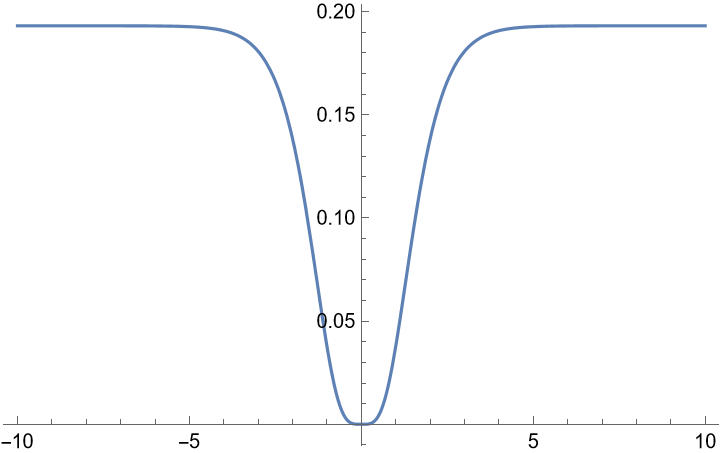
\includegraphics[width=\linewidth]{images/5c1.png}
                \caption{Graph of $H(u)$.}
                \label{fig1:a}
                \vspace{4ex}
            \end{subfigure}%%
            \begin{subfigure}[b]{0.5\linewidth}
                \centering
                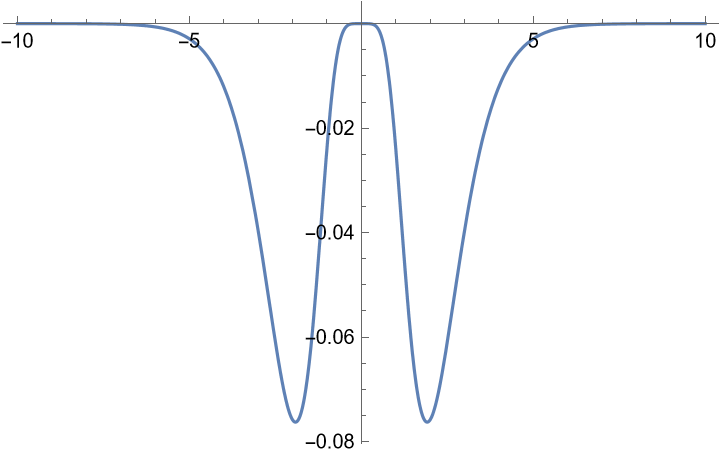
\includegraphics[width=\linewidth]{images/5c2.png}
                \caption{Graph of $H'(u)$.}
                \label{fig1:b}
                \vspace{4ex}
            \end{subfigure}
            \caption{Graphs of $H(u)$ and $H'(u)$}
            \label{fig1}
        \end{figure}

        \item[(d)]
        If $W$ is antisymmetric, then the bound $\dd{H}{t} \leq 0$ does not hold in general. For example consider when 
        \[ 
            W = \begin{bmatrix}
                0 & 1\\ -1 & 0
            \end{bmatrix} = - W^T,
        \]
        and $g(u_i) = \tanh(u_i)$. Then $H$ is given by
        \begin{align*}
            H =& -\frac{1}{2} \paren{0 + \tanh{u_1}\tanh{u_2} -\tanh{u_2}\tanh{u_1} + 0}\\ &+ \int_0^{\tanh(u_1)}\tanh^{-1}(V)\dt{V} + \int_0^{\tanh(u_2)}\tanh^{-1}(V)\dt{V},
        \end{align*} 
        and thus $H'$ is
        \begin{align*}
            \dd{H}{t} &= \tanh^{-1}(\tanh(u_1))(\tanh(u_1))'u_1' + \tanh^{-1}(\tanh(u_2))(\tanh(u_2))'u_2'\\
            &= u_1u_1'\text{sech}^2(u_1) + u_2u_2'\text{sech}^2(u_2)\\
            &= u_1(-u_1 + \tanh(u_2))\text{sech}^2(u_1) + u_2(-u_2 + \tanh(u_1))\text{sech}^2(u_2)
        \end{align*} 
        Thus we can see that $H'(u_1,u_2)$ is not less than or equal to zero for all $(u_1,u_2)$. For example, consider $H(0.25,5) = 0.31985 \not\leq 0$. Thus we no longer have the bound $\dd{H}{t} \leq 0$ when $W$ is antisymmetric.  

    \end{itemize}
\end{solution}

%----------------------------------------------------------------------------------------------------%
%\vskip 20pt
\newpage

%---------------%
%---Problem 6---%
%---------------%

%--status--$

\begin{problem}
    A specific case of the Lorenz equations is given by
    \begin{equation}
    \left\{\begin{array}{l}
    x^{\prime}=10(-x+y) \\
    y'=r x-y-x z \\
    z^{\prime}=-\frac{8}{3} z+x y
    \end{array}\right.
    \end{equation}
    \item [a] For varying r, find all equilibrium points and discuss
    their stability.
    \item [b] Calculate up to second order terms the local invariant manifolds $W^u$, $W^s$ and $W^c$
    for the fixed point at the origin of the Lorenz equations when $r=1$.
\end{problem}

\begin{solution}

    \noindent
    \begin{enumerate}
        \item [(a)]
        We consider the system
        \begin{equation*}
        \left\{\begin{array}{l}
        x^{\prime}=10(-x+y) \\
        y'=r x-y-x z \\
        z^{\prime}=-\frac{8}{3} z+x y
        \end{array}\right.
        \end{equation*}
        We can find the equilibrium points when $x' = y' = z' = 0$. Using Mathematica we can compute the fixed points to be:
        \begin{align*}
            \overline{(x,y,z)} \in & \left\{ (0,0,0), \left(-2 \sqrt{\frac{2}{3}} \sqrt{r-1},-2 \sqrt{\frac{2}{3}} \sqrt{r-1},r-1\right), \right. \\ & \left. \left(2 \sqrt{\frac{2}{3}} \sqrt{r-1}, 2 \sqrt{\frac{2}{3}} \sqrt{r-1}, r-1\right) \right\}.
        \end{align*}
        
        Next we can compute the Jacobian of the system to be
        \[ 
            J\begin{pmatrix}
                x\\y\\z
            \end{pmatrix} = \left(
                \begin{array}{ccc}
                 -10 & 10 & 0 \\
                 r-z & -1 & -x \\
                 y & x & -\frac{8}{3} \\
                \end{array}
                \right).
        \]
        Evaluating the Jacobian at the fixed point $(0,0,0)$ gives
        \[ 
            J\begin{pmatrix}
                0\\0\\0
            \end{pmatrix} = \left(
\begin{array}{ccc}
 -10 & 10 & 0 \\
 r & -1 & 0 \\
 0 & 0 & -\frac{8}{3} \\
\end{array}
\right),
        \]
        which has eigenvalues
        \[ 
            \lambda \in \left\{-\frac{8}{3},\frac{1}{2} \left(-\sqrt{40 r+81}-11\right),\frac{1}{2} \left(\sqrt{40 r+81}-11\right)\right\}.
        \]
        Using Mathematica we can determine that $\text{Re}(\lambda_i)<0$ when $r < 1$, which shows that the fixed point $(0,0,0)$ is asymptotically stable when $r<1$. Furthermore, when $r>1$, $\text{Re}(\lambda_i)>0$ which means that the fixed point is unstable. When $r=1$, $\text{Re}(\lambda_i)=0$ and thus the fixed point is undetermined in this case.

        Evaluating the Jacobian at the fixed point $\left(-2 \sqrt{\frac{2}{3}} \sqrt{r-1},-2 \sqrt{\frac{2}{3}} \sqrt{r-1},r-1\right)$ gives
        \[ 
            J\begin{pmatrix}
                -2 \sqrt{\frac{2}{3}} \sqrt{r-1}\\-2 \sqrt{\frac{2}{3}} \sqrt{r-1}\\r-1
            \end{pmatrix} = \left(
                \begin{array}{ccc}
                 -10 & 10 & 0 \\
                 1 & -1 & 2 \sqrt{\frac{2}{3}} \sqrt{r-1} \\
                 -2 \sqrt{\frac{2}{3}} \sqrt{r-1} & -2 \sqrt{\frac{2}{3}} \sqrt{r-1} & -\frac{8}{3} \\
                \end{array}
                \right),
        \]
        which has eigenvalues
        \begin{align*}
            \lambda \in &\big\{ \scriptscriptstyle -\frac{1}{9} \sqrt[3]{36 \sqrt{3} \sqrt{96 r^3+54119 r^2+91470 r-221310}+15012 r+5201}+\frac{8 r-\frac{961}{9}}{\sqrt[3]{36 \sqrt{3} \sqrt{96 r^3+54119 r^2+91470 r-221310}+15012 r+5201}}-\frac{41}{9},\\
            & \scriptscriptstyle \frac{1}{18} \left(1-i \sqrt{3}\right) \sqrt[3]{36 \sqrt{3} \sqrt{96 r^3+54119 r^2+91470 r-221310}+15012 r+5201}-\frac{\left(1+i \sqrt{3}\right) \left(8 r-\frac{961}{9}\right)}{2 \sqrt[3]{36 \sqrt{3} \sqrt{96 r^3+54119 r^2+91470 r-221310}+15012 r+5201}}-\frac{41}{9},\\
            & \scriptscriptstyle \frac{1}{18} \left(1+i \sqrt{3}\right) \sqrt[3]{36 \sqrt{3} \sqrt{96 r^3+54119 r^2+91470 r-221310}+15012 r+5201}-\frac{\left(1-i \sqrt{3}\right) \left(8 r-\frac{961}{9}\right)}{2 \sqrt[3]{36 \sqrt{3} \sqrt{96 r^3+54119 r^2+91470 r-221310}+15012 r+5201}}-\frac{41}{9}
             \big\}.
        \end{align*} 
        
        Using Mathematica we can determine that $\text{Re}(\lambda_i)<0$ when $1 < r < \frac{470}{19}$, which shows that the fixed point  $\left(-2 \sqrt{\frac{2}{3}} \sqrt{r-1},-2 \sqrt{\frac{2}{3}} \sqrt{r-1},r-1\right)$ is asymptotically stable when $1 < r < \frac{470}{19}$. Furthermore, when $r<1$ or $r > \frac{470}{19}$, $\text{Re}(\lambda_i)>0$ which means that the fixed point is unstable. When $r=1$ or $r=\frac{470}{19}$, $\text{Re}(\lambda_i)=0$ and thus the fixed point is undetermined in this case.

        Evaluating the Jacobian at the fixed point $\left(2 \sqrt{\frac{2}{3}} \sqrt{r-1}, 2 \sqrt{\frac{2}{3}} \sqrt{r-1}, r-1\right)$ gives
        \[ 
            J\begin{pmatrix}
                2 \sqrt{\frac{2}{3}} \sqrt{r-1}\\2 \sqrt{\frac{2}{3}} \sqrt{r-1}\\r-1
            \end{pmatrix} = \left(
                \begin{array}{ccc}
                 -10 & 10 & 0 \\
                 1 & -1 & -2 \sqrt{\frac{2}{3}} \sqrt{r-1} \\
                 2 \sqrt{\frac{2}{3}} \sqrt{r-1} & 2 \sqrt{\frac{2}{3}} \sqrt{r-1} & -\frac{8}{3} \\
                \end{array}
                \right),
        \]
        which has eigenvalues
        \begin{align*}
            \lambda \in &\big\{ \scriptscriptstyle -\frac{1}{9} \sqrt[3]{36 \sqrt{3} \sqrt{96 r^3+54119 r^2+91470 r-221310}+15012 r+5201}+\frac{8 r-\frac{961}{9}}{\sqrt[3]{36 \sqrt{3} \sqrt{96 r^3+54119 r^2+91470 r-221310}+15012 r+5201}}-\frac{41}{9},\\
            & \scriptscriptstyle \frac{1}{18} \left(1-i \sqrt{3}\right) \sqrt[3]{36 \sqrt{3} \sqrt{96 r^3+54119 r^2+91470 r-221310}+15012 r+5201}-\frac{\left(1+i \sqrt{3}\right) \left(8 r-\frac{961}{9}\right)}{2 \sqrt[3]{36 \sqrt{3} \sqrt{96 r^3+54119 r^2+91470 r-221310}+15012 r+5201}}-\frac{41}{9},\\
            & \scriptscriptstyle \frac{1}{18} \left(1+i \sqrt{3}\right) \sqrt[3]{36 \sqrt{3} \sqrt{96 r^3+54119 r^2+91470 r-221310}+15012 r+5201}-\frac{\left(1-i \sqrt{3}\right) \left(8 r-\frac{961}{9}\right)}{2 \sqrt[3]{36 \sqrt{3} \sqrt{96 r^3+54119 r^2+91470 r-221310}+15012 r+5201}}-\frac{41}{9}
             \big\}.
        \end{align*} 
        
        Using Mathematica we can determine that $\text{Re}(\lambda_i)<0$ when $1 < r < \frac{470}{19}$, which shows that the fixed point  $\left(-2 \sqrt{\frac{2}{3}} \sqrt{r-1},-2 \sqrt{\frac{2}{3}} \sqrt{r-1},r-1\right)$ is asymptotically stable when $1 < r < \frac{470}{19}$. Furthermore, when $r<1$ or $r > \frac{470}{19}$, $\text{Re}(\lambda_i)>0$ which means that the fixed point is unstable. When $r=1$ or $r=\frac{470}{19}$, $\text{Re}(\lambda_i)=0$ and thus the fixed point is undetermined in this case.

        \item [(b)]
        Next we wish to calculate up to second order terms the local invariant manifolds for the fixed point at the origin with $r=1$. First notice that the Jacobian evaluated at the origin is
        \[ 
            J\begin{pmatrix}
                0\\0\\0
            \end{pmatrix} = \left(
\begin{array}{ccc}
 -10 & 10 & 0 \\
 1 & -1 & 0 \\
 0 & 0 & -\frac{8}{3} \\
\end{array}
\right),
        \]
        which has the eigenpairs:
        \begin{align*}
            &\lambda_1 = -11, &&v_1 = \begin{bmatrix}
                -10\\1\\0
            \end{bmatrix},\\
            &\lambda_2 = -\frac{8}{3}, &&v_2 = \begin{bmatrix}
                0\\0\\1
            \end{bmatrix},\\
            &\lambda_3 = 0, &&v_3 = \begin{bmatrix}
                1\\1\\0
            \end{bmatrix}.\\
        \end{align*}
        Since $\text{Re}(\lambda_1),\text{Re}(\lambda_2) < 0$ they correspond to stable parts of the solution while $\text{Re}(\lambda_3) = 0$ corresponds to center part of the solution. Thus we are expecting \[\dim(W^u) = 0,~ \dim(W^s) = 2, \and \dim(W^c) = 1.\] 
        Now we introduce a coordinate transform
        \[ 
            \begin{pmatrix}
                u'\\v'\\w'
            \end{pmatrix} = T^{-1}AT \begin{pmatrix}
                u\\v\\w
            \end{pmatrix}  + T^{-1}R\left(T \begin{pmatrix}
                u\\v\\w
            \end{pmatrix}\right) = ,
        \]
        where $A = J((0,0,0)^T)$, $T=\left(
            \begin{array}{ccc}
             -10 & 0 & 1 \\
             1 & 0 & 1 \\
             0 & 1 & 0 \\
            \end{array}
            \right)$, and $R = (0,-xz,xy)^T$ which correspond to the nonlinear terms in the system of equations, thus we get
        \[ 
            \begin{pmatrix}
                u'\\v'\\w'
            \end{pmatrix} = \begin{pmatrix}
                -\frac{1}{11} v (w-10 u)-11 u\\(w-10 u) (u+w)-\frac{8 v}{3}\\\frac{-10}{11}  v (w-10 u)
            \end{pmatrix}.
        \]
        First let's find the local invariant stable manifold $W^s$. From class we know that we are searching for a polynomial of the form
        \[ 
            w = h(u,v),
        \]
        by the Implicit Function Theorem. Let's let $w$ be some general polynomial of the form
        \[ 
            h(u,v) = a u + b v + c u v + d u^2 + \rho v^2 + \dots
        \]
        and since the manifold is invariant we may take a derivative to get
        \begin{align*}
            \dd{w}{t} &= \pp{h}{u}\dd{u}{t} + \pp{h}{v}\dd{v}{t}.
        \end{align*} 
        We get the LHS to be
        \[ 
            \frac{1}{11} (-10) v \left(a u+b v+c u v+d u^2-10 u+\rho  v^2\right) + \dots
        \]
        and the RHS to be 
        \begin{align*}
            &(a+c v+2 d u) \left(-\frac{1}{11} v \left(a u+b v+c u v+d u^2-10 u+\rho  v^2\right)-11 u\right)\\ 
            &+(b+c u+2 \rho  v) \left(\left(a u+b v+c u v+d u^2-10 u+\rho  v^2\right) \left(a u+b v+c u v+d u^2+u+\rho  v^2\right)-\frac{8 v}{3}\right) + \dots.
        \end{align*} 
        We can drop the linear terms because there are none in $w'$ and thus $b = 0  \and a = 0$. We are also searching for a solution up to second order so we can toss out all the higher order terms. We can set the $uv$ term on the LHS equal to the one on the RHS to find that
        \[ 
           \frac{100}{11} = -11c - \frac{8}{3}c  \implies c = -\frac{300}{451}.
        \]
        Next we can set the $u^2$ term on the LHS equal to the one on the RHS to find that 
        \[
            -22u^2d = 0 \implies d = 0.
        \] 
        Next we can set the $v^2$ term on the LHS equal to the one on the RHS to find that 
        \[
            -\frac{16}{3}\rho = 0 \implies \rho = 0.
        \] 
        Thus we have found that 
        \[ 
            h(u,v) = - \frac{300}{451}uv + \dots,
        \]
        and transforming this back into cartesian coordinates using 
        \[ 
            \begin{bmatrix}
                u\\v\\w
            \end{bmatrix} = \begin{bmatrix}
                z\\ \frac{y - x}{11} \\ \frac{x + 10y}{11}
            \end{bmatrix}
        \]
        we find that the local invariant stable manifold $W^s$ is characterized by  
        \[ 
            \frac{x + 10y}{11} = -\frac{300}{451}(z)\paren{\frac{y-x}{11}} + \dots \implies x + 10 y + \frac{300}{451}(zy - zx) = 0 + \dots.
        \]

        Next let's find the local invariant center manifold $W^c$. To do so, let's consider the system of equations 
        \begin{align*}
            u &= h_1(w) = a_1 + b_1 w + c_1 w^2 + \dots,\\
            v &= h_2(w) = a_2 + b_2 w + c_2 w^2 + \dots.\\
        \end{align*}
        Since we know that the manifold passes through the fixed point $(0,0,0)$ and must be tangent to $E^c$, we can set $a_1 = b_1 = a_2 = b_2 = 0$ and since the manifold is invariant we can take a derivative to get
        \begin{align*}
            &\begin{cases}
                &u' = \pp{h_1}{w}\dd{w}{t} + \dots\\
                &v' = \pp{h_2}{w}\dd{w}{t} + \dots.    
            \end{cases}\\
            \implies &\begin{cases}
                -11c_1 w^2 - \frac{1}{11}c_2w^2(-10c_1w^2 + w) &= (2c_1w)(-\frac{10}{11}c_2w^2(-10c_1w^2 + w)) + \dots\\
                -\frac{8}{3}c_2w^2 + (-10c_1w^2 + w)(c_1w^2 + w) &= (2c_2w)(-\frac{10}{11}c_2w^2(-10c)1w^2 + w) + \dots
            \end{cases}
        \end{align*} 
        Since we are searching for solutions up to second order, let's drop all higher order terms yielding 
        \begin{align*}
            \begin{cases}
                &11c_1 w^2 = 0\\
                &-\frac{8}{3}c_2w^2 + w^2 = 0
            \end{cases} \implies \begin{cases}
                &-11c_1 = 0\\
                &-\frac{8}{3}c_2 + 1 = 0
            \end{cases} \implies \begin{cases}
                &c_1 = 0\\
                &c_2 = \frac{3}{8}.
            \end{cases}
        \end{align*}
        Thus we have found that 
        \begin{align*}
            \begin{cases}
                &v = \frac{3}{8}w^2\\
                &u = 0
            \end{cases}
        \end{align*}
        and transforming back into cartesian coordinates, we find that the local invariant center manifold is characterized by
        \[ 
            \begin{cases}
                &\frac{-x+y}{11} = \frac{3}{8}\paren{\frac{x+10y}{11}} + \dots\\
                &z = 0 + \dots
            \end{cases}
        \]
    \end{enumerate}
\end{solution}

%----------------------------------------------------------------------------------------------------%
%\vskip 20pt
\newpage

\end{document}